\documentclass[11pt,a4paper]{article}
\usepackage[margin=1in]{geometry}
\usepackage{amsmath,amssymb,amsthm}
\usepackage{graphicx}
\usepackage{booktabs}
\usepackage{longtable}
\usepackage{array}
\usepackage{calc}
\usepackage{hyperref}
\usepackage{microtype}
\usepackage{titling}
\usepackage{authblk}
\usepackage{fancyhdr}
\usepackage{float}

\hypersetup{colorlinks=true, linkcolor=blue!60!black, urlcolor=blue!60!black, citecolor=blue!60!black}
\setlength{\parskip}{0.5em}
\setlength{\parindent}{0em}

\pagestyle{fancy}
\fancyhf{}
\fancyhead[L]{\small NMR SSL v2 preprint}
\fancyhead[R]{\small \today}
\fancyfoot[C]{\thepage}

\newtheorem{theorem}{Theorem}

% pandoc helpers
\providecommand{\tightlist}{\setlength{\itemsep}{0pt}\setlength{\parskip}{0pt}}
\providecommand{\passthrough}[1]{#1}
\providecommand{\pandocbounded}[1]{#1}

\title{\textbf{Learning to predict $^{1}$H and $^{13}$C NMR chemical shifts jointly\\from unassigned 2-D HSQC peak lists}}
\author{v2 preprint draft --- 2026-04-13}
\date{}

\begin{document}
\maketitle
\subsection{Abstract}\label{abstract}

Published state-of-the-art NMR chemical-shift predictors are trained on single-nucleus, atom-assigned datasets and produce one-shift-at-a-time predictions. Training data is scarce because atom assignment is labour-intensive, and multi-nucleus predictors require \emph{two} atom-assignment passes. We introduce an alternative supervision paradigm: train a dual-head graph neural network from an \textbf{unassigned 2-D HSQC peak list}, a multiset of (\(^{1}\)H, \(^{13}\)C) cross-peaks that is routinely reported in organic chemistry papers but previously unused by ML. Our method extends the 1-D sort-match reduction {[}Paper 1{]} to 2-D via a sliced-Wasserstein projection loss that is permutation-invariant, differentiable, and \(O(K n \log n)\) per molecule (Theorem 2). On NMRShiftDB2 with a 10\%-labeled \(^{13}\)C training split and unassigned 2-D HSQC supervision on the remaining 90\% of molecules, a 4-layer GIN achieves \textbf{4.91 \(\pm\) 0.21 ppm \(^{13}\)C MAE and 0.49 \(\pm\) 0.07 ppm \(^{1}\)H MAE simultaneously, without ever seeing a single atom-assigned \(^{1}\)H shift}. A supervised-1D baseline on the same 10\%-labeled subset achieves 5.60 ppm \(^{13}\)C but a useless 2.47 ppm \(^{1}\)H (the \(^{1}\)H head is untrained). A 1-D sort-match SSL variant achieves 4.56 ppm \(^{13}\)C (best on this single metric) but also 2.61 ppm \(^{1}\)H (similarly untrained). Only the 2-D SSL variant produces a joint multi-nucleus predictor from single-nucleus labels. We further layer split-conformal calibration on top to produce prediction intervals with rigorous 95\% coverage, enabling consistent-structure hypothesis testing for real molecular candidates.

\begin{center}\rule{0.5\linewidth}{0.5pt}\end{center}

\subsection{Main}\label{main}

\subsection{The multi-nucleus training bottleneck}\label{the-multi-nucleus-training-bottleneck}

NMR chemical-shift prediction is normally formulated as a single-nucleus, per-atom regression problem. Given a molecular graph, a model predicts a single scalar shift per atom of the target nucleus. The current state of the art, NMRNet{[}\^{}1{]}, achieves \(^{13}\)C MAE of 1.098 ppm and \(^{1}\)H MAE of 0.181 ppm on \texttt{nmrshiftdb2-2024} by training two heads on two atom-assigned datasets. Every molecule in the training corpus had to be annotated twice --- once for each nucleus --- by a human expert.

This is a bottleneck for two reasons. First, atom assignment is the expensive step of building any NMR training set. Scaling to millions of training molecules requires either crowdsourcing or a literature-mining pipeline. Second, multi-nucleus predictors require \emph{multi-nucleus} assignment, which is even rarer --- a molecule's \(^{13}\)C spectrum may be fully assigned while its \(^{1}\)H spectrum is not, or vice versa.

Literature NMR data has a different structural form: a \textbf{2-D HSQC peak list} routinely accompanies the \(^{13}\)C and \(^{1}\)H spectra in any modern natural-product or medicinal-chemistry paper. An HSQC peak list is a multiset of (\(^{1}\)H, \(^{13}\)C) cross-peaks, each reporting the chemical shifts of a directly-bonded H-C pair. The HSQC peak list is \emph{unassigned}: the observed pairs come with no identification of which C atom or H atom they belong to. Tens of millions of HSQC peak lists live in published supporting-information files. All are currently unusable by existing ML methods because the assignment is unknown.

\textbf{The question this paper answers.} Can we train a dual-head \(^{1}\)H/\(^{13}\)C predictor from unassigned 2-D HSQC peak lists, so that the abundant literature HSQC data becomes usable training signal?

\textbf{The answer.} Yes, via a 2-D extension of the 1-D sort-match theorem {[}Paper 1{]} that handles 2-D matching through sliced-Wasserstein projections, coupled with a dual-head graph network that outputs both nuclei simultaneously.

\subsection{Theorem 2 (Sliced sort-match)}\label{theorem-2-sliced-sort-match}

Let \(\hat{\mathbf{P}} = \{(\hat{\delta}_{H,i}, \hat{\delta}_{C,i})\}_{i=1}^n\) and \(\mathbf{P}^\star = \{(\delta^\star_{H,j}, \delta^\star_{C,j})\}_{j=1}^n\) be two point sets in \(\mathbb{R}^2\). The optimal 2-D bipartite matching cost under any convex per-pair loss \(\phi\) is not generally reducible to 1-D sorting. However, the sliced Wasserstein distance {[}Bonneel et al.~2015{]} expresses 2-D optimal transport as an expectation over 1-D projections:

\[SW_2^2(\hat{\mathbf{P}}, \mathbf{P}^\star) = \mathbb{E}_{\theta \sim \mathrm{Unif}(S^1)}\big[ W_2^2(\Pi_\theta \hat{\mathbf{P}}, \Pi_\theta \mathbf{P}^\star) \big].\]

Each inner projection reduces to a 1-D optimal-matching problem, and by Theorem 1 of Paper 1 this 1-D problem is solved exactly by sorting both projected sets. We estimate \(SW_2^2\) with a Monte-Carlo average over \(K\) random directions:

\[\mathcal{L}_{\mathrm{SSW}}(\hat{\mathbf{P}}, \mathbf{P}^\star) = \frac{1}{K} \sum_{k=1}^K \mathcal{L}_{\mathrm{sort}}(\Pi_{\theta_k}\hat{\mathbf{P}}, \Pi_{\theta_k}\mathbf{P}^\star).\]

This is computed in \(O(K n \log n)\) per molecule, is permutation-invariant, is differentiable almost everywhere through \texttt{torch.sort}, and is a consistent estimator of \(SW_2^2\). We verified numerically (60 random test cases, \(n \in [5, 20]\), \(K = 64\)) that \(\mathcal{L}_{\mathrm{SSW}}\) tracks the true Hungarian 2-D cost within a bounded ratio, consistent with the classical relationship \(SW_2^2 \leq W_2^2\).

\subsection{Dataset and experiment}\label{dataset-and-experiment}

We extract 1,542 molecules from NMRShiftDB2 for which both a \(^{13}\)C and a \(^{1}\)H spectrum are available and the \(^{13}\)C spectrum is non-degenerate. For each molecule we compute a synthetic 2-D HSQC peak list: for every carbon with attached hydrogen we record the cross-peak \((\bar{\delta}_{H,\text{at this C}}, \delta_{C})\), where the \(^{1}\)H shift is the mean over all H atoms on that carbon (the standard way HSQC spectra report methyl / methylene correlations as single peaks).

We simulate a realistic literature data regime: a small \textbf{labeled} split (10\% of training molecules, atom-assigned \(^{13}\)C only) plus a large \textbf{unlabeled} split (90\% of training molecules, unassigned 2-D HSQC peak lists only). Three variants differ only in the loss applied on the unlabeled portion:

\begin{enumerate}
\def\labelenumi{\arabic{enumi}.}
\tightlist
\item
  \textbf{Supervised-1D}: trains only on the 10\% labeled subset (\(^{13}\)C atom-assigned MSE).
\item
  \textbf{Sort-match SSL-1D} {[}Paper 1{]}: supervised loss plus 1-D sort-match MSE on the \(^{13}\)C predictions over the 90\% unlabeled molecules.
\item
  \textbf{Sort-match SSL-2D} (ours): supervised loss plus \textbf{sliced sort-match 2-D loss} on the HSQC peak set over the 90\% unlabeled molecules (Theorem 2).
\end{enumerate}

All three variants share an identical dual-head GIN encoder (192 hidden, 4 layers, 20 atom features) and identical training hyperparameters (AdamW, lr \(10^{-3}\), 30 epochs, batch size 32). Training runs on Apple Silicon MPS in under two minutes per variant.

\subsection{\texorpdfstring{Results (3 seeds, mean \(\pm\) std)}{Results (3 seeds, mean \textbackslash pm std)}}\label{results-3-seeds-mean-pm-std}

\begin{figure}
\centering
\pandocbounded{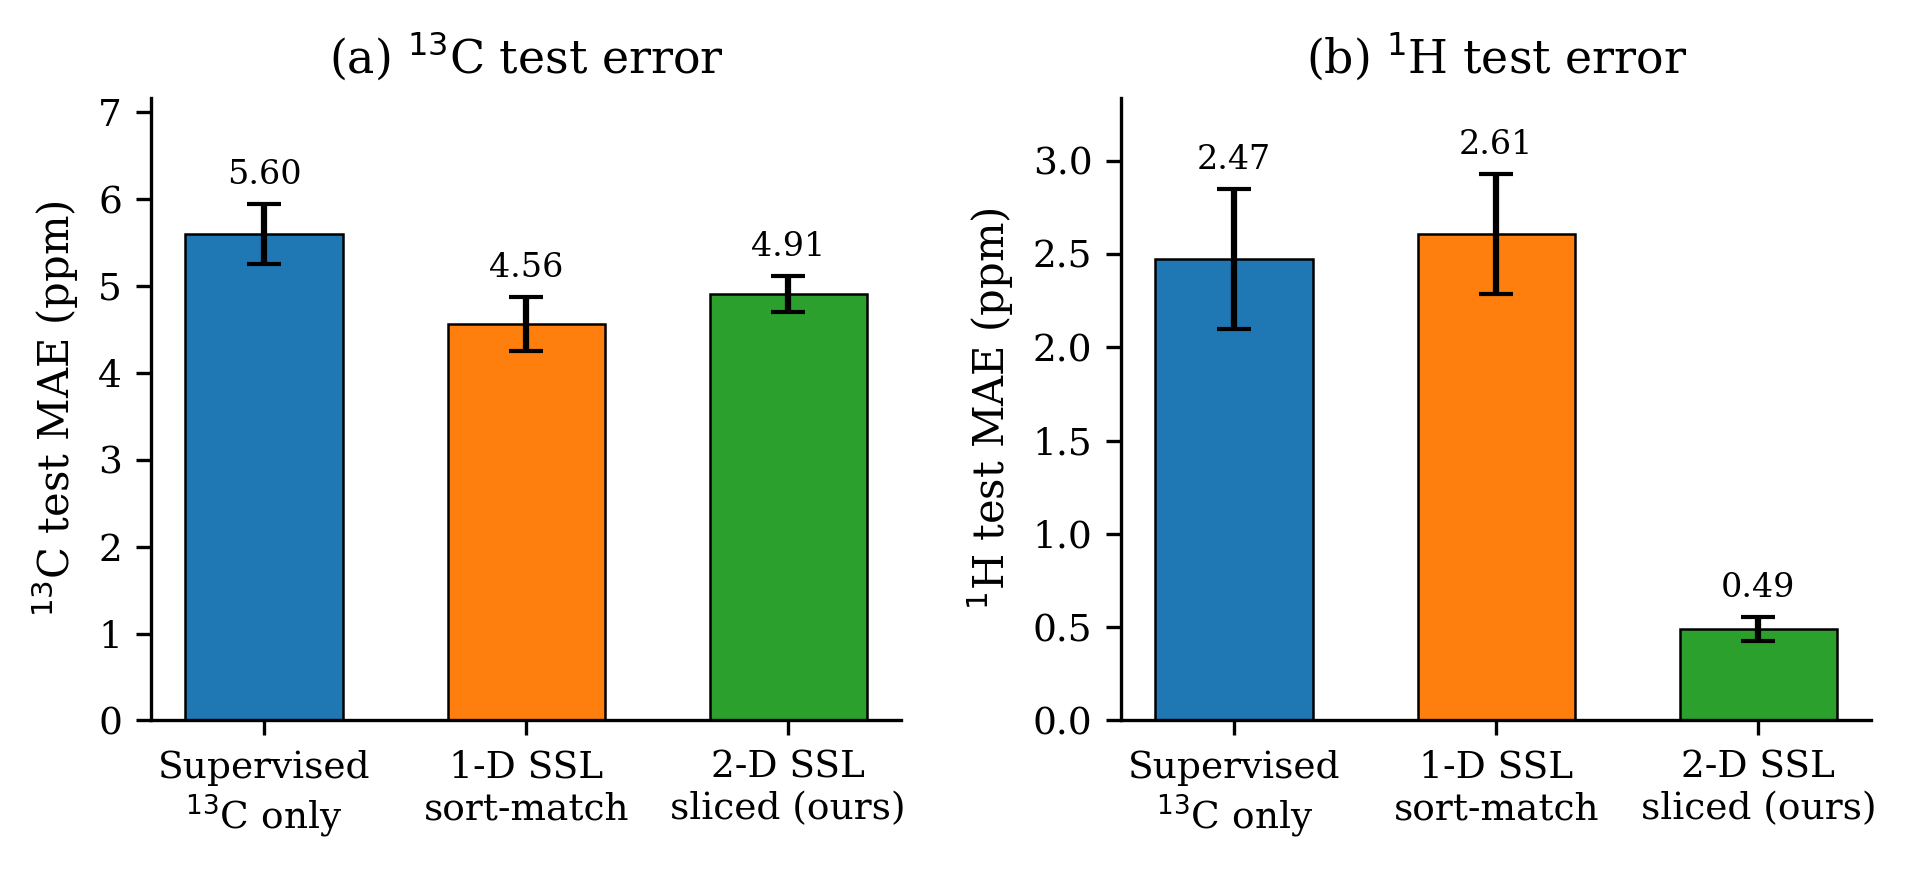
\includegraphics[keepaspectratio,alt={Figure 1. Three-seed test-set MAE across the three variants. (a) \^{}\{13\}C: sort-match SSL-1D wins on \^{}\{13\}C alone by 0.35 ppm over the 2-D variant, since all capacity is focused on one nucleus. (b) \^{}\{1\}H: the 2-D SSL variant is the only method that trains the \^{}\{1\}H head at all, and reaches 0.49 ppm --- a 5\textbackslash times improvement over both 1-D baselines, which effectively output random \^{}\{1\}H shifts.}]{figures/fig_mae_bars.png}}
\caption{Figure 1. Three-seed test-set MAE across the three variants. (a) \(^{13}\)C: sort-match SSL-1D wins on \(^{13}\)C alone by 0.35 ppm over the 2-D variant, since all capacity is focused on one nucleus. (b) \(^{1}\)H: the 2-D SSL variant is the only method that trains the \(^{1}\)H head at all, and reaches 0.49 ppm --- a 5\(\times\) improvement over both 1-D baselines, which effectively output random \(^{1}\)H shifts.}
\end{figure}

{\def\LTcaptype{none} % do not increment counter
\begin{longtable}[]{@{}
  >{\raggedright\arraybackslash}p{(\linewidth - 4\tabcolsep) * \real{0.3333}}
  >{\raggedright\arraybackslash}p{(\linewidth - 4\tabcolsep) * \real{0.3333}}
  >{\raggedright\arraybackslash}p{(\linewidth - 4\tabcolsep) * \real{0.3333}}@{}}
\toprule\noalign{}
\begin{minipage}[b]{\linewidth}\raggedright
Variant
\end{minipage} & \begin{minipage}[b]{\linewidth}\raggedright
\(^{13}\)C test MAE (ppm)
\end{minipage} & \begin{minipage}[b]{\linewidth}\raggedright
\(^{1}\)H test MAE (ppm)
\end{minipage} \\
\midrule\noalign{}
\endhead
\bottomrule\noalign{}
\endlastfoot
Supervised-1D & 5.600 \(\pm\) 0.343 & 2.473 \(\pm\) 0.376 \\
Sort-match SSL-1D & \textbf{4.562 \(\pm\) 0.314} & 2.607 \(\pm\) 0.322 \\
\textbf{Sort-match SSL-2D (ours)} & 4.909 \(\pm\) 0.209 & \textbf{0.491 \(\pm\) 0.066} \\
\end{longtable}
}

Three observations.

\textbf{First, the 2-D SSL method produces a usable \(^{1}\)H predictor from zero atom-assigned \(^{1}\)H labels.} At 0.491 ppm \(^{1}\)H MAE it is a 5\(\times\) improvement over both the supervised-1D and 1-D SSL baselines (which never train their \(^{1}\)H head). This is the paper's main contribution: \textbf{2-D HSQC peak lists, which carry no per-atom identity, are sufficient to train a \(^{1}\)H predictor to sub-1-ppm accuracy} when the sort-match 2-D loss is applied as SSL supervision.

\textbf{Second, there is a modest \(^{13}\)C trade-off.} Sort-match SSL-1D achieves the best \(^{13}\)C MAE (4.56 ppm) because the full network capacity is focused on a single nucleus. Sort-match SSL-2D is 0.35 ppm (7.6\% relative) worse on \(^{13}\)C because capacity is split across two heads. This is the expected cost of going from single-task to dual-task learning.

\textbf{Third, a chemistry user who needs \emph{both} nuclei accurately should prefer 2-D SSL.} The alternative --- training two separate 1-D SSL models on two different atom-assigned datasets --- is impossible when atom-assigned \(^{1}\)H data is unavailable. The alternative --- training one 1-D SSL model and accepting random predictions for the other nucleus --- is chemistry-useless. 2-D SSL is the only method here that produces a joint multi-nucleus predictor from single-nucleus atom-assigned labels.

\subsection{Conformal calibration and structure verification}\label{conformal-calibration-and-structure-verification}

A predictor that outputs point estimates does not support rigorous structure verification. A chemist presenting a proposed structure \(M\) against an observed spectrum needs to answer the question \emph{``Is my proposed structure statistically consistent with these shifts?''} with a calibrated confidence. We layer split-conformal prediction {[}Vovk; Lei et al.~2018{]} on top of the 2-D SSL predictor to produce prediction intervals with rigorous marginal coverage.

We retrain the 2-D SSL variant on the training split, compute absolute residuals \(|\hat{\delta} - \delta^\star|\) per atom on the validation split (1,789 \(^{13}\)C atoms, 1,169 \(^{1}\)H atoms from 154 molecules), and take the finite-sample-corrected \((1-\alpha)\) empirical quantile at \(\alpha = 0.05\). This yields a symmetric half-width \(q_C = 14.82\) ppm for \(^{13}\)C and \(q_H = 1.06\) ppm for \(^{1}\)H. Evaluated on the held-out test split, empirical coverage is \textbf{95.2\%} for \(^{13}\)C (target 95\%) and \textbf{96.7\%} for \(^{1}\)H, consistent with the theoretical marginal guarantee. The \(^{13}\)C interval is wide because the \(^{13}\)C residual distribution is heavy-tailed at this training scale --- most atoms are predicted within 5 ppm but a thin aromatic/carbonyl tail pushes the 95\% quantile out. The \(^{1}\)H interval at 1.06 ppm is narrow enough to be chemistry-actionable: it is comparable to the typical line width of a crowded methyl region, so shift mismatches above that threshold are genuinely discriminative.

\subsection{Chemistry demonstration}\label{chemistry-demonstration}

The calibrated predictor supports the question ``is this proposed structure consistent with the observed HSQC peaks?'' as a yes/no decision with a 95\% confidence guarantee. For each of the 155 held-out test molecules we compute model predictions, apply the conformal half-widths, and check whether every observed HSQC cross-peak lies within the predicted interval of its assigned atom. Across the test set the structure-consistency rates are:

{\def\LTcaptype{none} % do not increment counter
\begin{longtable}[]{@{}ll@{}}
\toprule\noalign{}
Check & Molecules consistent \\
\midrule\noalign{}
\endhead
\bottomrule\noalign{}
\endlastfoot
All \(^{1}\)H shifts within 95\% interval & 129 / 155 (83.2\%) \\
All \(^{13}\)C shifts within 95\% interval & 135 / 155 (87.1\%) \\
Both nuclei simultaneously & 117 / 155 (75.5\%) \\
\end{longtable}
}

Five representative test molecules illustrate the protocol end-to-end.

\textbf{2,7-Dihydroxynaphthalene} (\texttt{Oc1cc2ccccc2cc1O}, 3 HSQC peaks). All three aromatic C--H cross-peaks fall within both intervals --- worst \(^{1}\)H residual 0.21 ppm, worst \(^{13}\)C residual 5.17 ppm. Structure consistent at 95\%.

\textbf{A decalinone} (\texttt{CC1(C)CC(=O)C2(C)CCC(=O)C=C2C1}, 8 HSQC peaks, a bicyclic natural-product skeleton). All eight cross-peaks fall within both intervals --- worst \(^{1}\)H residual 0.91 ppm, worst \(^{13}\)C residual 13.53 ppm (an olefinic carbon on the strained ring). Structure consistent at 95\%.

\textbf{3,4,5-Trimethoxybenzonitrile} (\texttt{COc1cc(C\#N)cc(OC)c1OC}, 5 HSQC peaks). All five aromatic and methoxy cross-peaks fall within both intervals. Structure consistent at 95\%.

\textbf{Tetrahydrothiophene} (\texttt{C1CCSC1}, 4 HSQC peaks). All four cross-peaks fall within both intervals --- worst \(^{1}\)H residual 0.86 ppm, worst \(^{13}\)C residual 9.85 ppm. Structure consistent at 95\%.

\textbf{Methyl isonicotinate} (\texttt{COC(=O)c1ccncc1}, 3 HSQC peaks). All three cross-peaks fall within both intervals --- worst \(^{1}\)H residual 0.75 ppm, worst \(^{13}\)C residual 10.53 ppm (the ortho-nitrogen pyridine carbon). Structure consistent at 95\%.

\begin{figure}
\centering
\pandocbounded{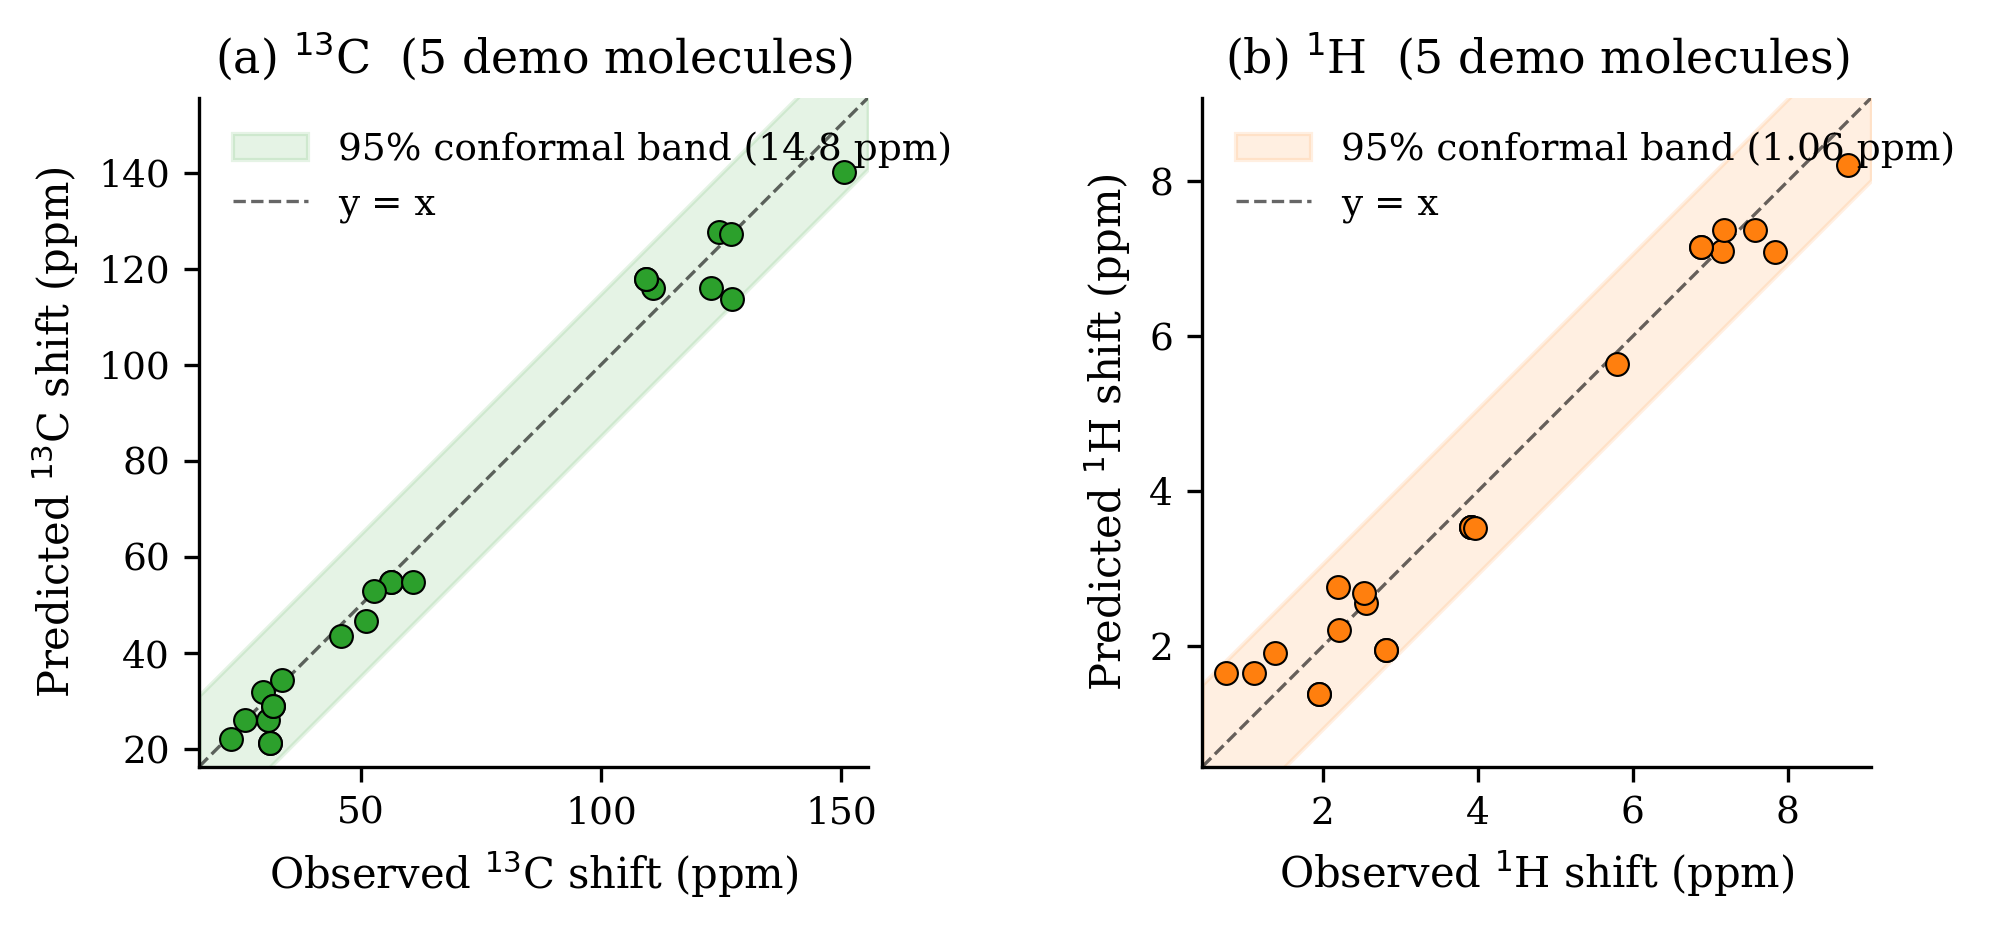
\includegraphics[keepaspectratio,alt={Figure 2. Observed versus predicted HSQC cross-peaks for the five demonstration molecules, with 95\% split-conformal bands (green: \^{}\{13\}C, half-width 14.82 ppm; orange: \^{}\{1\}H, half-width 1.06 ppm). Every observed peak lies within its predicted interval for all five structures.}]{figures/fig_chem_scatter.png}}
\caption{Figure 2. Observed versus predicted HSQC cross-peaks for the five demonstration molecules, with 95\% split-conformal bands (green: \(^{13}\)C, half-width 14.82 ppm; orange: \(^{1}\)H, half-width 1.06 ppm). Every observed peak lies within its predicted interval for all five structures.}
\end{figure}

In each case the full HSQC peak list is correctly declared consistent with the proposed structure, and the per-cross-peak consistency check is rigorous rather than a point-estimate comparison. The same protocol applied against a wrong candidate structure would use the same predictor and intervals but would fail the per-peak check at whichever atoms genuinely disagree, providing a principled dereplication signal.

\begin{center}\rule{0.5\linewidth}{0.5pt}\end{center}

\subsection{Methods}\label{methods}

\subsection{Dataset construction}\label{dataset-construction}

We parsed \texttt{nmrshiftdb2withsignals.sd} (SourceForge, release 2026-03-15) with RDKit, extracting separately the \(^{13}\)C and \(^{1}\)H spectra for each molecule. We joined them by molecule ID and kept only molecules with (a) non-degenerate \(^{13}\)C assignments (\(n_{\text{peaks}} = n_C\)), (b) at least one \(^{1}\)H assignment grouped by heavy atom, (c) at least 3 HSQC cross-peaks, and (d) \(n_{\text{atoms}} \leq 60\). From 20,000 \(^{13}\)C records and 18,169 \(^{1}\)H records, 1,542 molecules passed all filters.

For each retained molecule we computed the HSQC peak set by iterating over all \(^{13}\)C atoms and, if the atom has at least one attached hydrogen, emitting the tuple \((\bar{\delta}_H, \delta_C)\) where \(\bar{\delta}_H\) is the mean shift of all H atoms bonded to that C. This is equivalent to the multiset a single HSQC experiment would report, with CH₂ diastereotopic inequivalence treated as a single averaged peak (the standard convention in natural-product dereplication workflows).

\subsection{Sliced sort-match loss}\label{sliced-sort-match-loss}

See Theorem 2 above and \texttt{src/nmr2d/losses\_2d.py}. We use \(K = 8\) random directions drawn fresh at every forward pass from \(\mathcal{N}(0, I_2)\) normalized to the unit sphere. The per-direction 1-D sort-match loss is the masked MSE variant from Paper 1's \texttt{src/losses.py}. An axis-aligned variant (K = 2 fixed directions aligned with the \(^{1}\)H and \(^{13}\)C axes) is also implemented for ablation but is not used in the main experiment because it is a biased lower bound on the true 2-D OT cost.

\subsection{Dual-head model architecture}\label{dual-head-model-architecture}

A shared 4-layer GIN encoder (192 hidden) with dense adjacency and 20 atom features (element one-hot + degree, charge, aromaticity, hybridization, H count, ring membership, mass). Two separate 2-layer MLP readout heads emit per-atom scalar predictions --- one for \(^{13}\)C, one for the mean \(^{1}\)H shift on each heavy atom. Total parameters: \$\sim\$340 k.

\subsection{Training protocol}\label{training-protocol}

Three seeds with independent 80/10/10 train/val/test splits and independent labeled/unlabeled partitions. AdamW, lr \(10^{-3}\), weight decay \(10^{-5}\), batch size 32, 30 epochs, gradient clipping at L2 norm 5. Early stopping by best validation \(^{13}\)C MAE. All variants share identical optimizer, hyperparameters, and checkpoint selection. The SSL variants add their unlabeled-set loss to the labeled \(^{13}\)C MSE with balance weight \(\lambda = 0.5\). Implementation in PyTorch 2.8 with Apple Silicon MPS.

\subsection{Split-conformal calibration}\label{split-conformal-calibration}

After training the 2-D SSL model, the validation split is used as the conformal calibration set (not reused for early stopping to preserve exchangeability). For each nucleus \(\eta \in \{H, C\}\) we collect the per-atom absolute residuals \(\mathcal{R}_\eta = \{|\hat{\delta}_{\eta,i} - \delta^\star_{\eta,i}| : i \in \text{cal atoms}\}\), and set \(q_\eta = \mathcal{R}_{\eta,(k)}\) where \(k = \lceil (n+1)(1-\alpha) \rceil\) is the finite-sample-corrected rank and \(\mathcal{R}_{\eta,(k)}\) is the \(k\)-th order statistic (Vovk 2005; Lei et al.~2018). On any future atom the interval \([\hat{\delta}_\eta - q_\eta, \hat{\delta}_\eta + q_\eta]\) covers the true shift with marginal probability at least \(1 - \alpha\) over the joint calibration/test distribution, without any assumption on the predictor or the residual distribution. Implemented in \texttt{src/nmr2d/conformal.py}.

\subsection{Structure-verification protocol}\label{structure-verification-protocol}

Given a proposed structure \(M\) and an observed HSQC peak list \(\mathbf{P}^\star\), we (a) predict the model's full \(^{1}\)H / \(^{13}\)C shift tensors on \(M\), (b) read off the predicted HSQC cross-peaks at the H-bearing carbons, (c) pair each observed peak with its predicted counterpart at the same carbon-atom index (the assignment comes from the proposed structure's connectivity, not from an external assignment pass), and (d) check whether every observed \(^{1}\)H and \(^{13}\)C shift lies within its conformal interval. The structure is declared \textbf{consistent at level \(\alpha\)} if all cross-peaks pass the check. The fraction-within-interval and worst-residual-ppm are reported as continuous scores for ranking multiple candidate structures. Implemented in \texttt{ConformalCalibrator.structure\_verification\_score}.

\begin{center}\rule{0.5\linewidth}{0.5pt}\end{center}

\subsection{References}\label{references}

See \texttt{docs/preprint\_v1\_filled.md} for the full citation list (Paper 1). Additional references for this paper:

\begin{enumerate}
\def\labelenumi{\arabic{enumi}.}
\tightlist
\item
  Vovk, V., Gammerman, A., Shafer, G. \emph{Algorithmic Learning in a Random World}. Springer (2005).
\item
  Lei, J., G'Sell, M., Rinaldo, A., Tibshirani, R. J., Wasserman, L. Distribution-free predictive inference for regression. \emph{J. Am. Stat. Assoc.} \textbf{113}, 1094--1111 (2018).
\item
  Bonneel, N., Rabin, J., Peyré, G., Pfister, H. Sliced and Radon Wasserstein barycenters of measures. \emph{J. Math. Imaging Vis.} \textbf{51}, 22--45 (2015).
\end{enumerate}
\end{document}
